\section{Learning to Compute Strategic Solutions}
\label{sec:ai4gt}

When can the evidence in hand support a game-theoretic property claimed for a learned output, the \emph{claim question} (does it hold?) of
Section~\ref{sec:intro}? The answer depends on what the learner had access to, and
that access differs sharply across three settings. An equilibrium solver usually
starts from an explicit game or simulator, so it can evaluate any individual deviation, even when the full deviation class
is too large to exhaust. Strategic inference has less to work with: it observes play generated by
an unknown game, and different latent games can explain the same play equally
well. A learned mechanism is in between. It can be queried on types and misreports
before deployment, but publishing it can change who participates and
what they report afterward. Figure~\ref{fig:claim-obstacles} contrasts two recurring obstacles
that organize much of this section. Under
\emph{coverage}, the searched class is only part of the full
one, and a bound or more search must cover the rest. Under
\emph{identification}, distinct latent models fit the same play, and more data
cannot separate them. Throughout, the learned component supplies a candidate; what
certifies the property claimed for it is the surrounding argument, not the
learning. The rest of this section takes the three settings in
turn.

\begin{figure}[pos=t]
\centering
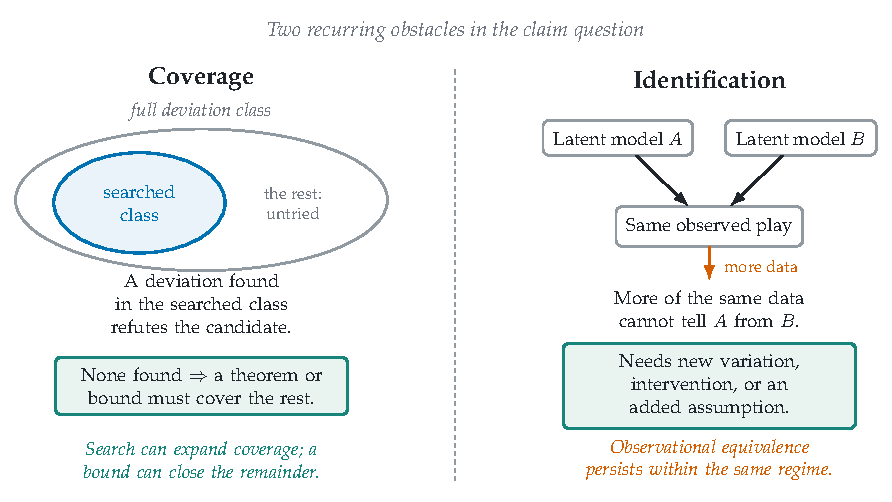
\includegraphics[width=\textwidth]{figure/fig5-claim-obstacles.pdf}
\caption{Two recurring obstacles in the claim question. \emph{Left (coverage):} the class
actually searched is a subset of the full deviation class; a deviation found there
refutes the candidate, but ruling out the rest needs a theorem or bound.
\emph{Right (identification):} two latent models can produce the same observed play,
and more of the same data cannot tell them apart --- only new variation,
intervention, or an added assumption can. Coverage recurs in equilibrium computation
(\S\ref{sec:ai4gt:equilibrium}), mechanism design (\S\ref{sec:ai4gt:mechanism}), and
strategic evaluation (\S\ref{sec:gt4ai:evaluation}); identification governs strategic
inference (\S\ref{sec:ai4gt:inference}) and joins coverage in deployment governance
(\S\ref{sec:gt4ai:governance}).}
\label{fig:claim-obstacles}
\end{figure}

\subsection{Equilibrium Computation with Learning}
\label{sec:ai4gt:equilibrium}

Take a solver computing a poker strategy. It can evaluate any specified bluff, but
the condition it must certify --- that \emph{no}
deviation pays --- ranges over the whole deviation class, far more than it can try.
That gap is the central tension of this subsection. Learned methods answer it by
pairing finite search with problem-specific analysis that controls what the search
left out; absent that analysis, the residual is measured only over the deviations
actually tried. We start from the classical baseline,
then cover learned quantities inside a solver, learned responses and
continuation values, and finally symbolic proposals that admit a direct check.

\subsubsection{Complexity and classical baseline}
The hardness results from the introduction apply to general finite games, but not
uniformly. Two-player zero-sum games (poker among them) occupy an easier regime, because their equilibrium conditions can be written as a matched pair of
linear programs, one per player. No-regret dynamics give a second route in: if two
players each drive their regret to zero, their average strategies approach the
minimax solution. This regret-to-equilibrium link is what the poker solvers later in
this subsection rely on, and it is special to two-player zero-sum play: it does not carry over unchanged to
general-sum games.

Classical numerical methods set the reference point. A fixed algorithm is already
reusable across explicitly represented games, though its computation is not
adapted from any training distribution. In a finite bimatrix game, support enumeration searches over possible supports
and solves the associated indifference and inequality conditions. The
Lemke--Howson algorithm recasts equilibrium as a linear complementarity
problem and pivots along a complementary path to a fully labeled
solution~\citep{LemkeHowson1964}. Homotopy methods embed the game in a
parameterized family and follow an equilibrium path from an easier auxiliary
problem. Gambit implements several of these
representations and algorithms~\citep{gambit}. All of them require finite, fully
represented games, and their worst-case cost stays substantial: Lemke--Howson can follow an
exponentially long path~\citep{SavaniVonStengel2006}.

\subsubsection{Learned quantities within equilibrium procedures}
When learning enters from inside the solver, it replaces a computed quantity ---
a response map, a value, a regret --- with a learned one. Each
method is therefore best assessed by the surrounding analysis: what it proves, for
which class of games, and to what target. Three sources of guarantee recur --- a direct
convergence proof, a regret bound, or, failing both, only empirical strength ---
and the target that can be certified weakens as the games leave the two-player
zero-sum case. Figure~\ref{fig:learning-substitution} lays out the three.

\begin{figure}[pos=t]
\centering
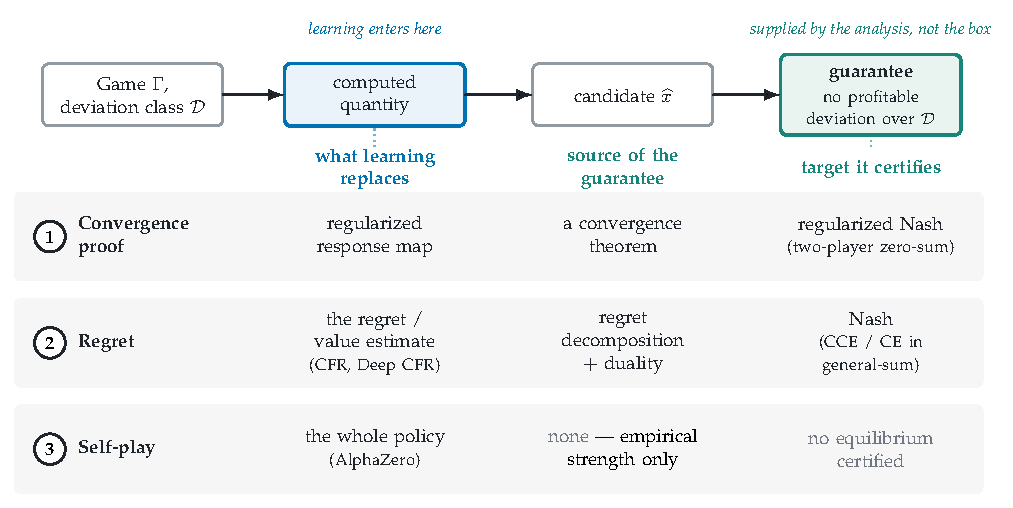
\includegraphics[width=\textwidth]{figure/fig3-learning-substitution.pdf}
\caption{Learning inside the equilibrium solver, and where the guarantee comes from.
The top row is the general shape of the claim question (cf.\
Figure~\ref{fig:claim-obstacles}): a learned quantity enters the solver, while a
separate convergence analysis, regret bound, or empirical evaluation determines
what can be claimed about the output. The three rows identify the learned
replacement, the supporting analysis, and the resulting target.
(Section~\ref{sec:ai4gt:equilibrium})}
\label{fig:learning-substitution}
\end{figure}

\runin{Guarantee from a convergence proof.} The first route smooths the response map, making it differentiable and therefore
amenable to policy-gradient and neural optimization. This smoothing, however,
shifts the target: any resulting guarantee applies to a regularized equilibrium
rather than the original equilibrium. \citet{NashPG2025} establish the strongest
such result. For an idealized refinement procedure, they prove that every step
strictly reduces the Bregman divergence to any Nash equilibrium and that the
procedure converges in two-player zero-sum extensive-form games. Yet this guarantee
applies to the idealized procedure, not to NashPG, the sampled algorithm used in
practice. \citet{LiuFarinaOzdaglar2025} expose the same limitation from another
angle by proving best-iterate convergence to a regularized equilibrium. Their result concerns only the best iterate (not every subsequent policy) and
only the regularized target. In both cases, the proof is substantive, but what it certifies
is narrower than the practical method built upon it.

\runin{Guarantee from regret.} The second route requires less machinery. Rather than proving convergence
directly, it derives the guarantee from regret. Once a learner's average regret
vanishes, no fixed deviation retains a persistent advantage in hindsight. In a
two-player zero-sum game, duality converts this into a bound on the exploitability
of the average strategy. Counterfactual regret minimization (CFR) extends the idea
to extensive-form games by decomposing the overall regret across information
sets~\citep{Zinkevich2007}. It is this decomposition, rather than a separate
argument, that yields the exploitability bound.

This guarantee is exact but tabular. Scaling it beyond an explicit table degrades
it, though in a controlled manner. Deep CFR replaces the tabular regrets with
neural approximations~\citep{BrownDeepCFR2019}, so that sampling and
function-approximation error enter the same exploitability bound through the same
regret decomposition. The guarantee is therefore not lost but widened, by an error
term the analysis makes explicit.

\runin{No equilibrium guarantee: self-play.} Return-maximizing self-play without an
equilibrium-residual objective offers no equilibrium guarantee from training alone.
It can achieve strong play, as AlphaZero shows, without ever minimizing an
equilibrium residual. It provides empirical evidence of performance against the
training population, which may hide a profitable counterstrategy or permit
cycling among mutually exploitable policies. Methods that do certify an equilibrium
require an analysis connecting the training objective or stopping rule to the stated
target, for example through a controlled equilibrium residual or response-oracle
condition.

Every route so far has assumed two-player zero-sum play, where the target is
unambiguous. In general-sum games it is not, and the certifiable guarantee weakens
accordingly. Independent external-regret minimization now reaches only the coarse
correlated equilibria (CCE); stronger internal- or swap-regret guarantees reach
the correlated equilibria (CE). The two differ by deviation class: a coarse
correlated equilibrium rules out committing to a fixed action before observing a
recommendation, whereas a correlated equilibrium also rules out deviations that
condition on it. Both are weaker than Nash equilibrium, since neither requires the
joint distribution to factorize into independent strategies. The weaker target is
also computationally cheaper: these equilibria admit linear descriptions and are
verifiable in polynomial time. It remains, however, a different target, since
reaching a coarse correlated equilibrium does not solve the original Nash problem.
Meta-learned CFR treats this residual gap as its objective, training a
parameterized regret minimizer whose meta-loss measures the distance remaining to
the stronger Nash condition~\citep{Sychrovsky2025}.

\subsubsection{Learned responses for empirical games}
The previous route assumed the solver could work with the game itself: evaluate deviations, form regrets,
invoke duality. That assumption breaks when the game is
given only by a simulator, its normal form too large to enumerate. Empirical
game-theoretic analysis proceeds anyway. It approximates the game by a finite policy
population: the analyst picks a strategy set, estimates its payoffs by simulation,
and solves the resulting empirical game~\citep{WellmanTuylsGreenwald2025}. The
guarantee question shifts with the setting. It is no longer whether an analysis
certifies a learned quantity, but whether the population covers the deviations that
matter. The methods below are two ways of growing and solving that population, each
leaving its own coverage gap.

\runin{Response-oracle expansion.} Policy-space response oracles (PSRO) grow the
population adaptively~\citep{Lanctot2017}. They solve the current empirical game,
train an approximate best response to its meta-strategy, add that policy, and
estimate the new payoff entries. A multi-agent reinforcement learner supplies the
response oracle; the empirical-game solver coordinates the policies already found.
Pipeline PSRO runs several such response processes and empirical-game updates
concurrently for scale~\citep{McAleerPipelinePSRO2020}. What the population certifies
is only as strong as the responses the oracle can find.

\runin{Correlated-equilibrium meta-solvers.} Joint policy-space response oracles
(JPSRO) keep the population structure but change the solution concept used for the
empirical game~\citep{Marris2021}. At each iteration a deep reinforcement-learning oracle
searches for responses to a distribution drawn from the empirical game. Max-Gini
selection then picks a high-entropy correlated or coarse correlated equilibrium
among the solutions. The output is a CE or CCE of the empirical game: the same retreat to a weaker
target seen for general-sum games above, now driving population
growth rather than relaxing a regret bound.

Carrying any of these solutions back to the underlying game requires accurate payoff
estimates and coverage of deviations outside the current population. Here the finite
empirical game is not one ingredient of the solver but an approximation standing in
for the underlying game, and the quality of that approximation sets what the solution
supports.

\subsubsection{Learned continuation values for online re-solving}
The last two routes changed what the computation runs on: shared across
instances, or a population standing in for the game. This route keeps the game exact
and changes instead \emph{when} the computation runs. Large imperfect-information
games can postpone work until play reaches a subgame. A solver builds a coarse
blueprint offline and re-solves the current subgame online, which injects extra
exploitability at the subgame boundary. What holds that error in check is the
organizing question, and the answer tracks how much of the continuation is learned
rather than computed exactly. Three systems span the range.

\runin{Bounded learned values.} DeepStack keeps the continuation learned and bounds
the resulting error~\citep{Moravcik2017}. In heads-up no-limit poker it continually
re-solves the public portion of the game, calling a neural counterfactual-value
function beyond a limited lookahead. The network thus compresses continuation
computation across public states, while continual re-solving and
counterfactual-value bounds hold the added exploitability in check. The learned
value is what is deferred; the bound is what certifies it.

\runin{Exact safe re-solving.} Libratus reaches the same end with no learned value
at all~\citep{BrownSandholm2018}. It combines a CFR-based blueprint with nested safe
subgame solving and endgame refinement, its safe-resolving component carrying no
neural approximation. This marks the exact end of the range: the boundary
exploitability is controlled by construction, not by a bound on a learned object.
That control is precisely what DeepStack's value network trades away for scale.

\runin{Reformulation with a convergence proof.} ReBeL neither bounds a learned value
nor forgoes learning; it reformulates the game so that a proof becomes
available~\citep{BrownReBeL2020}. Each public belief state pairs public information
with a distribution over the players' private states. This yields a
continuous-state, perfect-information game on which reinforcement learning and
search can operate. Trained through self-play as policy and value networks, ReBeL is
used inside nested subgame solving. For two-player zero-sum games, it admits a proof
of convergence to Nash equilibrium under the prescribed representation and solving
assumptions. Private information stays hidden: the public belief state is all the
recursion needs.

Across the range, the boundary guarantee comes from the re-solving analysis --- a
value bound, a safe-resolving construction, or a convergence proof --- not from the
learned value alone. Figure~\ref{fig:learning-substitution} draws the same
separation for the equilibrium pipeline. What moves along the range is only how much
of the continuation is entrusted to learning.

\subsubsection{Symbolic proposals under executable checks}
The routes so far attached a guarantee to a learned numerical object --- a value, a
regret, a response --- and bounded its error. This route breaks that dependence. A generator proposes a symbolic object (an equation, or code) for an
individual game, and a separate formal or computational component checks feasibility and the
relevant deviation conditions. Provided the encoding and checker are sound, the
mechanical test establishes the property whatever produced the proposal. That is
what makes an unreliable generator, such as a language model, tolerable. The two
methods below differ only in the level of the generated object: a solution, or the
algorithm that produces one.

\runin{Generating a solution.} PrimeNash targets analytical equilibrium
characterization for an individual game~\citep{PrimeNash2025}. Its agents generate
candidate strategies and symbolic derivations, then call executable tools to
manipulate and test the expressions. The target is an instance-specific symbolic
characterization, parameter regions and boundary cases included. The guarantee
comes from explicit best-response conditions and machine-executable checks, not
from the generator.

\runin{Generating an algorithm.} LegoNE moves the generation one level up, to the
synthesis of equilibrium algorithms~\citep{LegoNE2025}. Expert proof strategies
live in a domain-specific language. Each generated algorithm is compiled into a
finite constrained optimization problem, whose solution determines a worst-case
approximation guarantee for the encoded game class and objective. The check is now
a bound on the algorithm, not a test of one solution.

Across the four learned routes, the guarantee comes from elsewhere than the
learning. Where it is deductive, it rests on the
surrounding analysis: duality, regret decomposition, safe resolving, or verified
constrained optimization. Where it is not, as in empirical games, the claim is only
as strong as the population's coverage. Total cost includes data generation and
training, and any residual approximation should be reported as exploitability or
regret.

\subsection{Strategic Inference: What Observed Play Can Identify}
\label{sec:ai4gt:inference}

The previous subsection ran the pipeline forward: a known game in, a
certified strategy out, the obstacle one of coverage that more search can close.
Strategic inference runs it backward. Watching only realized play (a bidder's bids, or players' moves), it must
recover the game that produced them, with no game
given in advance. Its obstacle is different in kind. Two different valuations can
explain the same bids equally well, and more data from the same auction cannot tell
them apart. This is an identification limit, not a
coverage one: it yields to informative variation or maintained restrictions, never
to sample size alone.

Two questions must be settled in order, and either can fail. The first is
falsifiability: could \emph{any} data prove the model wrong? Often not.
\citet{HaileHortacsuKosenok2008} show that QRE is so flexible that it can fit
any pattern of behavior in a single game. QRE is the model in which players
usually choose better actions but sometimes err, and the result survives even
under strong restrictions on the unobserved noise. A model that fits any observation
has no testable implication on its own: QRE acquires identifying content only when
further assumptions are added, such as a
response rule that stays fixed as the game changes.

The second question is recoverability: granting a falsifiable model, is the latent
quantity pinned to a point? Often it is not. In multi-agent inverse reinforcement
learning, one observed equilibrium is usually consistent with many reward functions.
For the entropy-regularized class they study, \citet{FreihautRamponi2025} show that
a given reward induces a unique quantal response equilibrium. This removes the
equilibrium-selection ambiguity but does not collapse the feasible reward set to a
point. What remains is an identified set, its width recording the leftover
ambiguity. Only informative variation narrows it: cross-game or within-participant
variation can separate explanations that coincide along a single realized path. The
model restrictions decide which differences would be informative, and the data must
actually contain them.

Against this backdrop, learned methods differ mainly in where they insert the
assumption that makes identification possible. Three groups do so at three places:
in a learned response model, in a fixed one, or in a search over candidate models.
Table~\ref{tab:inference_methods} sets the three side by side.

\begin{table}[pos=t]
\centering
\caption{Where learned strategic-inference methods insert the assumption that makes
identification possible. (Section~\ref{sec:ai4gt:inference})}
\label{tab:inference_methods}
\footnotesize
\setlength{\tabcolsep}{3.5pt}
\renewcommand{\arraystretch}{1.25}

\begin{tabularx}{\textwidth}{
    >{\raggedright\arraybackslash}p{0.15\textwidth}
    >{\raggedright\arraybackslash}p{0.20\textwidth}
    Y
    Y
    Y
}
\toprule
\textbf{Assumption location}
& \textbf{Representative methods}
& \textbf{Identifying assumption}
& \textbf{What it recovers}
& \textbf{Remaining limitation}
\\
\midrule

Learned response model
& GameNet~\citep{Hartford2016}, ElementaryNet~\citep{DEon2026ElementaryNet}, and
cognitive-model pretraining~\citep{Bourgin2019}
& The network's architecture or its pretraining data encodes the behavioral theory
& A predictive response model fit to the observed play
& Matching predictions does not validate the model's internal behavioral
interpretation
\\

\addlinespace

Fixed model, estimated latents
& A differentiable equilibrium layer~\citep{Ling2018}, dominance-based
intervals~\citep{CuiYu2023}, and a generative relation model~\citep{Shum2019}
& A specified game plus restrictions --- dominance, regularization --- on the unknowns
& Payoffs, types, or relations, as a point, a set, or a posterior
& Only as sharp as the restrictions; often an identified set, not a point
\\

\addlinespace

Search over symbolic models
& AutoBM~\citep{AutoBM2026}
& A hypothesis space of models and a held-out fit criterion
& A symbolic model that fits the data
& Models with equal fit stay indistinguishable; the whole compatible set should be
carried forward
\\

\bottomrule
\end{tabularx}
\end{table}

\runin{Learning the response model.} The first group lets the network carry the
behavioral theory. GameNet maps a two-player normal-form payoff matrix to a
distribution over actions~\citep{Hartford2016}. Its architecture is symmetric under
relabeling the actions, with layers meant to capture non-strategic (level-$0$) play
and a few rounds of players responding to one another. ElementaryNet exposes a hidden ambiguity in that
design: GameNet's nominal level-$0$ component can itself express strategic
responses~\citep{DEon2026ElementaryNet}. Replacing it with one formally unable to do
so, then adding explicit higher-level modules, recovers statistically
indistinguishable predictive performance. Matching predictions therefore does not
validate the behavioral interpretation of a model's internal parts. A related strategy instead supplies the theory through the training data,
pretraining on synthetic choices from cognitive models before fine-tuning on human
observations~\citep{Bourgin2019}.

\runin{Estimating latent quantities in a fixed model.} The second group fixes the
response model and estimates the hidden quantities inside it: the payoffs, private types, or
relationships among agents that the model treats as unknown. The output may
be a single estimate, a feasible set, or a full posterior, and the methods differ in
what they can identify. A differentiable regularized-equilibrium layer passes
prediction error back to the game's parameters~\citep{Ling2018}. In auction data,
dominance restrictions turn observed bids into intervals of possible valuations,
which then enter the loss of a learned bidding model~\citep{CuiYu2023}. A generative
model of social relations instead supports Bayesian inference over the latent
relationships~\citep{Shum2019}.

\runin{Searching over symbolic models.} The third group searches the model itself.
AutoBM proposes symbolic response models in natural language and code, compiles and
fits them, and selects by held-out likelihood~\citep{AutoBM2026}. But selection
still depends on observed fit. Models that predict the same observations stay
indistinguishable, so downstream decisions should account for the whole compatible
set, not treat the selected model as identified.

Across the three groups, the identifying power is exactly the assumption inserted
--- a network's inductive bias, a fixed model's structure, or a search's admissible
class --- and none of it is supplied by the data. Where the assumptions leave the
latent quantity underdetermined, what the data support is the identified set, and a
conclusion is trustworthy only if it holds across that whole set.

\subsection{Mechanism Design: Learning Rules under Incentive Constraints}
\label{sec:ai4gt:mechanism}

Consider a learned auction. Unlike strategic inference, which only watches, the
designer can feed the mechanism any bid before deployment and see how it responds; the access strategic inference lacked is restored. Yet the mechanism faces two tests
at once: its incentive properties before deployment, and its performance after. The
first test is unforgiving. Incentive compatibility (IC) requires truthful bidding to
beat every misreport, for every bidder type, including bids that never appeared in the sample. Finite training and evaluation establish that only when a theorem or
bound controls the omitted cases. It helps to separate two senses of ``outside the training
distribution,'' because they are not the same kind of problem:

\begin{itemize}
\item From \emph{sampled truthful type profiles} to the deployment type
distribution. This affects objectives computed in expectation (revenue, welfare) and is the
ordinary generalization problem.
\item From \emph{searched misreports} to all profitable deviations. This affects
the incentive claim itself, and it is not an averaging problem: a single
unexamined misreport that pays is a counterexample, not a tail event.
\end{itemize}

The gap from searched misreports to all profitable deviations is what the incentive
claim turns on. Write
\(u_i(v_i, b_i, b_{-i})\) for the utility of agent \(i\) whose true type is
\(v_i\), who reports \(b_i\), and whose opponents report \(b_{-i}\). The first
argument is the true type; the remaining arguments are the submitted reports.
For a direct mechanism, dominant-strategy incentive compatibility then
requires truthful reporting to dominate every misreport:
\[
u_i(v_i,v_i,b_{-i})
\;\geq\;
u_i(v_i,b_i',b_{-i}),
\]
for all agents \(i\), all types \(v_i\), all alternative reports \(b_i'\), and
all opponent profiles \(b_{-i}\). The condition is counterfactual: it weighs truthful reporting against
alternative reports, including ones that may never
appear in the training data. A single profitable misreport shows the mechanism is
not incentive compatible; establishing that it \emph{is} requires the inequality
to hold over the entire type and misreport spaces.

That asymmetry organizes the methods. During training, an optimizer or misreporter
network can submit alternative reports to the candidate mechanism and score their
utility on sampled types. From there the approaches fork: some minimize the
resulting empirical regret in a flexible mechanism class; others restrict the
representation, or add post-training analysis, to cover the full type and report
spaces. Shared parameters let allocation and payment computations be reused across
type profiles, and the remaining costs come from the representation and from
checking beyond the training sample. The parts below organize the methods by where the incentive claim rests: in explicit
constraints, in the empirical regret from searched violations, or in the mechanism's construction.

\subsubsection{Guarantees from explicit constraints: the classical baseline}

Automated mechanism design provides the computational baseline. In a finite type
space, a designer introduces allocation and payment variables for each reported
type profile and optimizes expected revenue or social welfare. Feasibility,
individual rationality, and incentive compatibility enter as explicit linear or
mixed-integer constraints~\citep{ConitzerSandholm2002,CurryAMDSurvey2025}.

The virtue of the direct formulation is also its limit. The number of allocation
and payment variables grows with the cardinality of the agents' joint type space,
and incentive compatibility adds comparisons between truthful and alternative
reports on top. Continuous types usually force discretization, and the resulting
program enforces the constraints only at the chosen grid points unless a further argument controls behavior between them: finer grids shrink
that error while enlarging the program.

\subsubsection{Guarantees from searched violations: incentive compatibility as a loss}

Neural mechanism design trades the table of type-contingent outcomes for
parameterized allocation and payment functions, and turns incentive compatibility
into a quantity to minimize. Two moves recur: make the regret itself the training
loss, or vary the architecture and objective around that loss.

\runin{Regret as the training loss.} RegretNet is the central instance of the
move~\citep{Duetting2019}. Given a reported valuation profile, one network outputs
an allocation and another the payments. The parameters are trained to maximize
expected revenue while controlling violations of incentive compatibility and
individual rationality. For bidder \(i\), ex-post regret at a valuation profile is
\[
r_i(v)
=
\max_{b_i'}
\left[
u_i(v_i,b_i',v_{-i})
-
u_i(v_i,v_i,v_{-i})
\right].
\]
The mechanism is incentive compatible exactly when this is zero for every bidder at
every valuation profile. RegretNet estimates the maximization through gradient-based
searches over misreports, and folds the resulting regret into an augmented-Lagrangian
objective. The shape is a two-player contest: the mechanism network proposes
allocations and payments, and an inner search returns profitable misreports as both
violation and training signal. ALGNet makes the inner player explicit, replacing the
optimization with a learned misreporter~\citep{Rahme2021Auction}. It evaluates regret
over the deviations that misreporter can represent and find. The auctioneer changes
the mechanism to raise revenue; the misreporter searches for reports that raise an
agent's utility.

\runin{Variants on architecture and objective.} The remaining methods keep empirical
regret but reshape what surrounds it. RegretFormer adds attention and an explicit
regret budget, giving admissible empirical regret a direct role in the
objective~\citep{Ivanov2022}. EquivariantNet exploits bidder and item permutation
symmetries to share computation across relabeled
instances~\citep{Rahme2021Equivariant}. CITransNet extends the transformer
formulation to contextual and variable-scale auctions, its permutation-equivariant
architecture accommodating varying numbers and attributes of
participants~\citep{Duan2022}. PreferenceNet changes the objective instead, learning
fairness- and diversity-related constraints from representative
examples~\citep{Peri2021}. None of these moves establishes incentive compatibility
for unseen reports: the supporting evidence stays empirical, regret evaluated on
sampled types and searched misreports.
Table~\ref{tab:ic_location_mechanism_design} sets this basis against methods that
place the incentive property in the representation or in post-training analysis.

\begin{table}[pos=t]
\centering
\caption{Where incentive compatibility resides in learning-based mechanism design.
(Section~\ref{sec:ai4gt:mechanism})}
\label{tab:ic_location_mechanism_design}
\footnotesize
\setlength{\tabcolsep}{3.5pt}
\renewcommand{\arraystretch}{1.25}

\begin{tabularx}{\textwidth}{
    >{\raggedright\arraybackslash}p{0.13\textwidth}
    >{\raggedright\arraybackslash}p{0.20\textwidth}
    Y
    Y
    Y
}
\toprule
\textbf{IC location}
&
\textbf{Representative methods}
&
\textbf{Source of IC evidence}
&
\textbf{Main benefit}
&
\textbf{Remaining limitation}
\\
\midrule

External constraints
&
Classical automated mechanism design~\citep{ConitzerSandholm2002,CurryAMDSurvey2025}
&
Explicit incentive-compatibility, individual-rationality, and feasibility constraints in a linear or mixed-integer optimization problem
&
Directly represents the economic constraints and permits exact optimization in finite type spaces
&
The number of variables and constraints grows rapidly with the type space; continuous types require discretization
\\

\addlinespace

Differentiable loss
&
RegretNet~\citep{Duetting2019}, ALGNet~\citep{Rahme2021Auction}, and RegretFormer~\citep{Ivanov2022}
&
Empirical ex-post regret evaluated against misreports found through gradient-based optimization or a learned misreporter
&
Supports flexible neural allocation and payment rules and scalable gradient-based training
&
Low empirical regret is limited to the sampled types and the misreports found by the search
\\

\addlinespace

Architectural inductive bias
&
EquivariantNet~\citep{Rahme2021Equivariant}, CITransNet~\citep{Duan2022}, and PreferenceNet~\citep{Peri2021}
&
Permutation equivariance, attention-based contextual representations, or learned auxiliary design constraints, combined with empirical regret evaluation
&
Improves generalization across relabeled, contextual, or variable-scale auction instances
&
Architectural structure alone leaves incentive compatibility unproved for unseen reports
\\

\addlinespace

Truthful representation
&
MenuNet~\citep{Shen2019}, RochetNet~\citep{Duetting2019}, and AMenuNet~\citep{Duan2023}
&
Bidder-optimal menu selection or the dominant-strategy incentive compatibility of an affine-maximizer mechanism
&
Inherits incentive properties from the economic representation; learning selects within that family
&
Restricting the mechanism to a structured family may exclude better-performing mechanisms outside that family
\\

\addlinespace

Structure and checking
&
GemNet~\citep{Duetting2024}, BundleFlow~\citep{WangBundleFlow2025}, truthful mechanisms without discretization~\citep{TEDI2025}, and LLM-AMD~\citep{LiuGuoConitzer2025}
&
Menu-compatibility conditions, post-processing, regularity bounds, truthful pricing architectures, or verification of executable mechanism code
&
Links the learned rule to explicit structural or verification conditions
&
Requires additional assumptions, restricted representations, post-processing procedures, or computationally costly verification
\\

\bottomrule
\end{tabularx}
\end{table}

\subsubsection{Guarantees by construction: menus and affine maximizers}

A cleaner alternative makes truthfulness structural. Confine the learned mechanism
to a family whose economic form already supports honest behavior, and no regret
penalty is needed to enforce it. The illustrative case is a menu: it lists
allocation--payment pairs, and a bidder picks the option that maximizes its utility
at its true valuation, so the designer need not learn a separate outcome for every
report. The methods below carry this construction from one bidder to many, and then
to outcome spaces too large to enumerate.

\runin{Single-bidder menus.} MenuNet searches over such menus for single-bidder
environments~\citep{Shen2019}. RochetNet parameterizes a utility or menu
representation built around the characterization of truthful single-bidder
mechanisms~\citep{Duetting2019}. In both, the network optimizes the quality of the
menu while bidder-optimal selection supplies the economic basis for truthfulness.
Approximation may affect how close the revenue comes to optimal, but the source of
the incentive guarantee is the structure, not an empirical regret penalty.
\FloatBarrier

\runin{Multi-bidder affine maximizers.} Affine-maximizer auctions give the
multi-bidder analogue. An affine maximizer picks an allocation by maximizing a
weighted sum of reported valuations plus allocation-specific offsets. With the
matching payment rule, it inherits dominant-strategy incentive compatibility and
individual rationality from the construction. AMenuNet learns the weights, offsets,
and a scalable set of candidate allocations, rather than searching unrestricted
allocation and payment functions~\citep{Duan2023}. The neural model widens the
practical search over affine-maximizer mechanisms, while the classical mechanism
class fixes the strategic property. Restricting the representation may exclude the
unconstrained revenue-optimal mechanism, but any candidate inside the class inherits
its basic truthfulness from the construction, with no empirical regret minimization.

\runin{Scaling the construction.} Scaling to general multi-bidder auctions raises a
compatibility problem. Each bidder can be seen as facing a menu conditioned on the
others' reports, and those menus must jointly correspond to a feasible allocation
and payment rule. GemNet formalizes this menu-compatibility
requirement~\citep{Duetting2024}. Its training penalizes compatibility violations,
and its post-training construction adjusts prices so the learned menus define a
strategy-proof mechanism, with Lipschitz regularity bounding the error from checking
only a finite valuation grid. BundleFlow pushes menu learning into combinatorial
auctions, where the item space is far larger~\citep{WangBundleFlow2025}. An
unrestricted menu there is exponentially large, since every subset of items can
define a distinct option. BundleFlow instead uses a learned flow- or diffusion-based
procedure to generate the relevant bundles and their menu entries, without
enumerating the full bundle space. Bidder-optimal selection keeps the generated menu
truthful, while the omitted bundles and learned prices set its approximation error.
A different frontier removes discretization from the outcome space entirely:
\citet{TEDI2025} parameterize pricing rules with Partial GroupMax Networks, an
architecture that admits only rules satisfying the stated truthfulness conditions
over continuous outcomes, so training merely selects among them.

\subsubsection{Guarantees that can be re-checked: executable mechanisms}

A deployable mechanism has to specify a rule whose feasibility and incentive properties can actually be analyzed, which is easiest when the rule
is code.
LLM-AMD formulates automated mechanism design as the generation of mechanism
code~\citep{LiuGuoConitzer2025}. A language model proposes an executable rule from
a natural-language description of the environment and objective. A
problem-specific fixing process then revises the candidate to address feasibility
and strategy-proofness violations. It can recover canonical auction structures and
produce redistribution rules in the settings considered, and, through
programming-by-example, can re-express a previously learned neural mechanism as a
more interpretable program. Making the rule executable makes its failures easier to inspect and search for, but the rule can still
violate a constraint on an untested input.

Publishing a mechanism also changes the environment it acts on. Participant
responses can alter entry and the reports observed after deployment, so the
deployment distribution of reports may drift from the sampled training
distribution. The mechanism does not thereby identify the underlying type
distribution; endogenous participation or type formation needs an explicit model
of its own.

\subsection{From the Claim Question to the Goal Question}
\label{sec:ai4gt:bridge}

Across its three settings, this section asked one question: does a learned output
really have the strategic property claimed for it, the \emph{claim question}
(does it hold?) of Section~\ref{sec:intro}? In the results surveyed here, access
repeatedly imposed the two limits set out at the start of the section. Equilibrium
computation and mechanism design met a \emph{coverage} gap: a poker solver can
evaluate any specified bluff, and an auction can be fed any bid before deployment,
yet the bluffs and bids are too many to exhaust, so a theorem or a bound has to cover
the ones left untried. Strategic inference centered on an \emph{identification} gap, which
yields only to a new kind of variation or an added assumption, never to more of the
same data. The two call for different remedies, and broader search does nothing for
the second.

One thing held throughout: the learned object was judged against a reference that does not react to it: a fixed game, a fixed
dataset, a fixed set of bidders. Real
deployments break that assumption. A published auction changes who shows up and what
they bid; a pricing algorithm, once live, moves the very market it is judged in.
Section~\ref{sec:gt4ai} turns to this world. Once the object acts, its opponents, its
training counterpart, and the market all respond, and the question changes. It is no
longer whether the output has its property, but whether that property --- proved
inside a designed game --- delivers the real goal the game was meant to capture. A
pricing rule can be verified to maximize its own firm's profit and still fail the
market outcome a regulator cares about. That is the \emph{goal question} (does it help?) of Section~\ref{sec:intro}.
